\RequirePackage{fix-cm}
\documentclass[smallextended]{svjour3}       % onecolumn (second format)
\smartqed  % flush right qed marks, e.g. at end of proof
\usepackage{graphicx,multicol,lipsum,caption,authblk} \usepackage{amsmath,booktabs,verbatim,tikz}
\usepackage{geometry,pgf,pgfplots,}
\usepackage{mathptmx}
\usetikzlibrary{shapes.geometric, arrows,positioning,matrix,calc}
\usetikzlibrary{intersections}
\bibliographystyle{unsrtnat}
% in order to solve arranging citations by order of appearance
\usepackage[numbers]{natbib}
\usepackage{notoccite}
\begin{document}


\title{Parameters Study of Sharing Mechanism on Genetic Algorithm for Multimodal Problem}
%\titlerunning{Stacking Sequence Optimization}        % if too long for running head
\author{Zhang Huiyao$^1$  \and
	Atsushi Yokoyama $^{1,*}$
}
\authorrunning{Zhang Huiyao} % if too long for running head
\institute{Zhang Huiyao \at
              Room 203,Bulding 3,Kyoto Institue of Technology\\
			  Matsugasaki,Sakyo-ku,Kyoto,606-8585,JAPAN\\
              \email{zhanghy1012@gmail.com}           %  \\
           \and
           S. Author \at
              second address
}
\date{Received: date / Accepted: date}
\maketitle

\begin{abstract}
    Sharing mechanism is widely used in genetic algorithm (GA) to solve
    multimodal problems.  In this paper, the influenece of parameters of share
    function on the search performance of GA is studied. There are three key
    factors in the share function, which are metric space, distance constant and
    index constant. First, the metric space is studied based on the peroformance
    of GA; second the distance constant is determined based on optimal metric
    space; finaly,According to the metric space and distance constant, the index
    constant is decided. According to the five criterias of the experiment, the
    optimal combination of these three parameters are determined to maxmize the
    performance of GAs.
\keywords{Genetic Algorithm \and Niche \and Metric Space \and Multimodal}
\end{abstract}

\begin{multicols}{2}

\section{Introduction}
Genetic algorithms (GAs) are first introduced in 1975 by
Holland\cite{sampson1976adaptation}, because of its powerful search ability,
which was widely been used to solve many search, optimiation, and classification
problem. Compared with other random search algorithm, for example, particle
swarm optimization, ant colony optimization, and simulated annealing
algorithm\cite{zabinsky2010random}, GAs are not easily trapped in local optima,
and obtain the global optimal.  Traditional GAs has been to successfully find
the optimal value in the domain for unimodal problems, however, sometimes, not
only the optimal point but also the secondary important point is needed.
Because of its search rule, traditional GAs are failed to maintain the
information for a multimodal problem.


\subsection{Genetic Algorithm Procedure}
According to Darwin natural evolution theory, the one who fits the environment
most well are more possilbe to survive and reproduction. GA simulates the
process of natural evolution which includes selection,crossover and mutation.
Because of the powerful search ability of GA,it has been widely used in many
fields for multimodal problems. The procedure diagram of GA as shown in figure
\ref{plot:GA} 
 
\subsection{Parent Selection}
Selection is the most important step of GA algorithm which decides the diversity
of the population. In the step, if the selection pressure increase, the converge
speed of the population increase, however, the diversity of the dopulation
decrease. To improve the search ability and reduce the search cost,
many selection methods \cite{goldberg1991comparative} has been invented,the
selection schemes can be divided into four classes which are proportionate
reproduction, ranking selection, tournament selection and Genitor(or "steady
state") selection.In this paper, to maintain a stable subpopulation for
multimodel problems,the stochastic remainer algorithm is used for experiment,
stochastic remainder algorithm is one of proportional selection method according
to corresponding fitness.

\subsection{Parents Crossover}
According to the selected parents, crossover is used to generate the offspring,
combining genes from parents to reproduce new members. There are so many
research \cite{ahmed2010genetic,nebro2009mocell} about the crossover operation
in GAs to maximize the divistiy of the population. In this paper, one-point
crossover strategy is implemented.

\subsection{Offspring Mutation}
Mutation simulates the situation  genes on the chromosomes which received from
parents randomly changed.  The process are used to provide new evolution
direction and information for the population, the parameters has during this
process has been well researched by Schaffer\cite{schaffer1989study}.  


\subsection{Niched Mechanism}
Niched mechanism simulates another natural process of subpopulation in the
evolutionary process, and introduce the concept niches which means sharing
resource.  Because GA select the best individual according to their fitness, so
the GA converges quickly to find the global optimal value. Howerver, In order to
deal with the multimodal problem, It is significant to maintain the diversity of
the population.  Niched mechanism simulates the There are several methods to
achieve this target,which are Crowding, Deterministic Crowding and Sharing
methods.  share Function\cite{goldberg1987genetic}. In this paper, the
parameters of share function is studied. 
\begin{center}
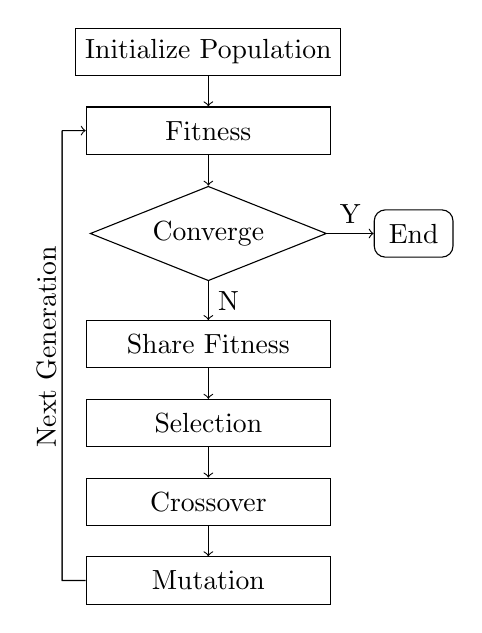
\begin{tikzpicture}
\tikzstyle{startstop} = [rectangle, rounded corners, minimum width=1.0cm,minimum height=0.6cm, 
                        text centered, draw=black]
\tikzstyle{io} = [trapezium, trapezium left angle=70, trapezium right angle=110, minimum width=2cm, 
                 minimum height=0.6cm, text centered, draw=black]
\tikzstyle{process} = [rectangle, minimum width=3.1cm, minimum height=0.6cm, text centered, draw=black]
\tikzstyle{decision} = [diamond,minimum width=3cm, minimum height=1.2cm, draw=black]
\node (population) [process] {Initialize Population};
\node (fitness) [process, below of=population] {Fitness};
\node (decision) [decision] at ($(fitness.south)+(0,-1.0cm)$) {} node at (decision.base) {Converge};
\node (share-fitness) at ($(decision.south)+(0,-0.8cm)$) [process] {Share Fitness};
\node (selection) [process,below of=share-fitness] {Selection};
\node (crossover) [process,below of=selection]  {Crossover};
\node (mutation) [process,below of=crossover]   {Mutation};
\node (end) [startstop] at ($(decision.east)+(1.1cm,0)$)  {End};
\draw [->] (population) -- (fitness);
\draw [->] (fitness) -- (decision);
\draw [->] (decision) -- (share-fitness) node[auto=left,pos=0.5]{N};
\draw [->] (share-fitness.south) -- (selection.north) ;
\draw [->] (selection.south) -- (crossover.north);
\draw [->] (crossover.south) -- (mutation.north);
\draw [->] (decision.east) -- (end.west) node[auto=left,pos=0.5]{Y};

% draw intersection
\draw [white] (fitness.west) -- ++(-0.5cm,0) coordinate (A);
\draw [white] (mutation.west) -- ++(-0.3cm,0) coordinate (B)-- ++(0,6cm) coordinate (C) ; 
\draw (mutation.west) -- ++(-0.3cm,0) -- (intersection cs: first line={(fitness.west)--(A)}, 
      second line={(B)--(C)}) coordinate (D);
\draw (B) -- (D) node[auto=left,pos=0.8,rotate=90,xshift=-0.2cm,yshift=0.2cm] {Next Generation} ;
\draw [<-] (fitness.west) -- (D);
\end{tikzpicture}
\captionof{figure}{GA Procedure with Share Function}
\label{plot:GA}
\end{center}

\subsection{Sharing}
Sharing mechanism is first introduced by Holland \cite{miller1996genetic} to
reduce the fitness of similar individual in the population and increase the
diversity of the population. For Sharing mechanism, the most important thing is
how to identify the number of niches, Miller comed up dynamic niche sharing
method, and lin developed the method to identify the number of niches in the
population.\cite{lin2002niche}

\subsection{Shareing Issue}
The problem within sharing mechanism is how to identiy the range of parameters
in the formula. Given the number of peaks in population,Deb and Goldberg comed
up method to set up the appropriate value for $\sigma_{sh}$, however,in many
problems, the number of peaks is difficult to identify, and more often, the
fitness is discrete. So it is important to determine these parameters properly.
\begin{equation}
s h\left(d_{i, j}\right)=\left\{\begin{array}{ll}{1-\left(\frac{d_{i, j}}{\sigma_{s h}}\right)^{\alpha_{s h}}} 
    & {\text { if } d_{i, j}<\sigma_{s h}} \\ 
{0} & {\text { otherwise }}\end{array}\right.
\end{equation}




\section{Research Method}
According to the following share function
$$
\begin{aligned} 
\operatorname{sh}(\mathrm{d}) & = 1 - \left(\frac{\mathrm{d}}{\sigma_{\text {share }}}\right)^{\alpha}, 
                                  \quad \mathrm{d}<\sigma_{\text {share }} \\ 
                              & = 0, \quad \text { otherwise }
\end{aligned}
$$
where $d$ denotes distance between two strings, $\alpha$ is a contant number,
$\sigma_{\text {share}}$ is also a constant number.

define share fitness $f_i^{\prime}$ as the following


where $m_i^{\prime}$ indicates niche count,

%\begin{equation}

%    m_i^{\prime}=3

%\end{equation}


\begin{equation}
d_{ij} = d(x_i,x_j)
\end{equation}

There are three factors which influence the performance of GAs, which are metric
space and two constant numbers.  Metric space is one of the most important
factors which influence the effect of GA.  Suppose $x_i$ and $x_j$ denotes two
different string in the population. Given the metric space $(M,d)$, metric
function $d$ is: $$d: M\times M \rightarrow R$$
This can be divided into the following three steps, the first is the
normalization of metric space.

1: Metric Normalization

In order to discuss the influence of different parameters, the normalization of
metric distance is necessary, suppose $d_{max}$ means the longest distance
between two strings in the population, So the distance can be normalized by the
following formula:
\begin{equation}
d_{norm} = \frac{d_i}{d_{max}}
\end{equation}

After normalization the distance between any two points is:
\begin{equation}
    0 \leq d_{ij}\leq 1 
\end{equation}


2: Define Tensor

Define $D$ and $D^{\ast}$ as the basic metric space and dual metric space, which
can be used as the basic building block to define all the metric space, and a
tensor with $r$ basic metric space and $q$ dual metric space is defined as by
the formula:

\begin{equation}
    D = |x_i-x_j|
\end{equation}

\begin{equation}
    D^{\ast} = \sqrt{|x_i-x_j|}
\end{equation}

\begin{equation}
t(r,s):= \underbrace{D \bigotimes \cdots \bigotimes D}_{r} \times \underbrace{D^{\ast} \bigotimes 
\cdots \bigotimes D^{\ast}}_{s} \rightarrow R
\end{equation}
where $R$ stands for real number.

3: constant $d_{share}$ in share formula


Given the best tensor condition, increase the value of $d_{share}$ to check the
influence of d on the search ability of GAs.take the step length $d_{step}=0.5$,
after the nomalization of metric space, the distance $d_{max}$ between two
points in M satisfiy $d_{max}\leq 1$. According to the share function theory,
$d_{share}$ needs great then $d_{max}$. So the range of is $\{d_{share}|d > 1\}$

 


\section{Experiment and Results}

\subsection{Experiment Method}
1. GA

In order to evaluate the impact of the parameters, the mutation process is
ignored. The parameters of GA is shown in the table \ref{tab:GA}

\begin{center}
\captionof{table}{GA-parameters}
\begin{tabular}{cc}
	\toprule
	parameter & value \\
	\midrule
	population size      & 50 \\
    encoding method      & binary encoding\\
    encoding length      & 16 \\
	selection strategy   & roulette wheel  \\
	crossover strategy   & one-point \\
	mutation strategy    & None \\
	\bottomrule
\end{tabular}
\label{tab:GA}
\end{center}


The ith individual in the population converted  from binary to decimal by the
following formula:

\begin{equation}
x_i=\frac{\sum_{j=1}^{16}2^{j-1}g_i^j}{2^{15}}
\end{equation}


2. Evaluation indexes

To evaluate the performance of GA algorithm, four index are come up. The first
evaluation criterion is apparent reliability denoted as $R$, which is calulate
by the following formula
\begin{equation}
R = \frac{n}{\text{N}}
\end{equation}
$n$ stands for the number of GA finds at least one optimal point, $N$ stands for
the number of the runtime of GA.
The second criterion is the normalized cost of GA,denoted as $C_n$,which is
calculated by the following equation:
\begin{equation}
C_{n} = N_{g}P/R
\end{equation}
where P is population size.  The third criterion is population richness, denoted
as $P_{r}$, which is calculated by the following formula:
$$
P_{r} = N/P
$$
Population richness is used to denote how many optimal points these GA
maintains.  The fourth criterion is the number of best output, denoted by
$O_{n}$.  The last criterion is the number of niche, denoted by $N_{n}$, the
number of niche can be used to represents the ability of the GA to maintain
subpopluation.


\subsection{Result}
Example 1:

\begin{equation}
f_{1}(x)=\sin^{6}(5.1 \pi x+.5)
\end{equation}

The experiment result in the table \ref{tab:tensor}, with $d_share$ equals 2 and the value of $\sigma$ 
is 1.

\begin{center}
    \captionof{table}{$\alpha_{sh}$}
\begin{tabular}{cccccc}
	\toprule
    $\alpha_{sh}$& $R$ & $C$ & $O_{n}$ & $P_{r}$ & $N_{n}$\\
	\midrule
    1/3  & 0.96  & 2094.24 & 3.21 & 10.82  & 4.50 \\
    1/2  & 0.93  & 2150.54 & 3.08 & 9.26  & 4.41 \\
    1    & 0.96  & 2094.24 & 3.29 & 7.76  & 4.47 \\
    2    & 0.95  & 2116.40 & 3.04 & 7.13 & 4.47 \\
    3    & 0.93  & 2150.53 & 2.48 & 6.99 & 4.40 \\
	\bottomrule
\end{tabular}
\label{tab:tensor}
\end{center}

According to the table \ref{tab:tensor}, with the sum of $r+s$ increases, the
population richness $P_r$, The number of best output $O_n$ and the number of
niches $N_n$ decrease,and when $r=1$ and $q=0$,apparent reliability R obtain the
maximaize value,GA obtains the best result.  as shown in Fig.
\ref{fig:sin-result} 

\begin{center}
  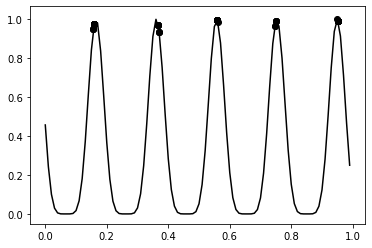
\includegraphics[width=\linewidth]{GA_images/example-sin-result.png}
  \captionof{figure}{Result 1}
  \label{fig:sin-result}
\end{center}

2. niche radius influence under tensor $t(1,0)$

Because $t(1,0)$ obtain the best search result,

\begin{center}
\captionof{table}{$d_{share}$ parameter}
\begin{tabular}{cccccc}
	\toprule
    $r_{niche}$ & $R$ & $C$ & $O_{n}$ & $P_{r}$ & $N_{n}$\\
	\midrule
    1.1 & 0.98 & 2040 & 4.08 & 12.24 & 5.42 \\
    1.6 & 0.98 & 2040 & 5.10 & 13.36 & 5.52 \\
    2.1 & 0.98 & 2040 & 5.18 & 12.06 & 5.12 \\
    2.6 & 1.0  & 2000 & 5.16 & 10.2 & 4.66 \\
    3.1 & 0.98 & 2040 & 4.70 & 9.32 & 4.44 \\
    3.6 & 0.96 & 2083 & 4.5  & 8.22 & 4.12 \\
    4.1 & 0.98 & 2040 & 4.86 & 8.44 & 4.18 \\
	\bottomrule
\end{tabular}
\label{tab:d-share}
\end{center}

\begin{center}
  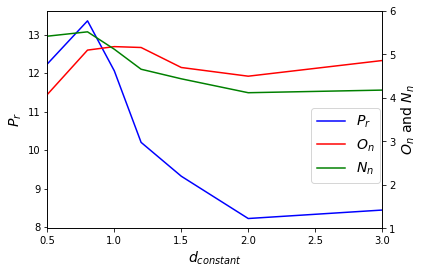
\includegraphics[width=\linewidth]{GA_images/d_constant.png}
  \captionof{figure}{niche radius}
  \label{fig:d-share}
\end{center}

According to Tab \ref{tab:d-share},  we can see that when $d_{share}=1.6$,
the performance of GA is best; Combined with Fig.\ref{fig:d-share}, when 
$$1.1 \leq d_{share} \leq 2.1$$

The GA performed the best.


3. power index influence

\captionof{table}{$\sigma$ parameter}
\begin{tabular}{cccccc}
	\toprule
    $\sigma$ & $R$ & $C$ & $O_{n}$ & $P_{r}$ & $N_{n}$\\
	\midrule
    0.5 & 0.98 & 2040 & 4.64 & 13.02 & 5.08 \\
    0.8 & 0.92 & 2173 & 4.56 & 13.08 & 5.22 \\
    1.0 & 0.98 & 2040 & 5.10 & 13.36 & 5.52 \\
    1.2 & 0.98 & 2040 & 5.32 & 11.72 & 5.36 \\
    1.5 & 0.96 & 2083 & 4.80 & 9.80 & 4.68 \\
    2.0 & 0.96 & 2083 & 3.94 & 7.50 & 4.10 \\
    3.0 & 0.96 & 2083 & 2.08 & 3.58 & 2.34 \\
	\bottomrule
\end{tabular}

\begin{center}
  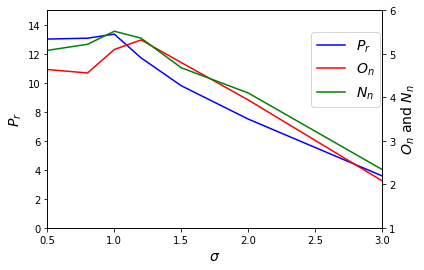
\includegraphics[width=\linewidth]{GA_images/sigma-parameter.png}
  \captionof{figure}{$\sigma$ parameter}
  \label{fig:sigma}
\end{center}

Example 2:

$$
\mathrm{f}_{2}(\mathrm{x})=\mathrm{f}_{1}(\mathrm{x}) \cdot \mathrm{e}^{\left[-4 \ln 2 \frac{(\mathrm{x}-0.086)^{2}}{0.8^{2}}\right]}
$$

%$$
%f_{1}(x)=\cos^{6}(5.1 \pi x+.5)
%$$


\captionof{table}{Metric Space Example}
\begin{tabular}{cccccc}
	\toprule
    Metric & $R$ & $C$ & $O_{n}$ & $P_{r}$ & $N_{n}$\\
	\midrule
    $t(1,0)$ & 1.00 & 2000 & 4.98 & 11.6 & 4.94 \\
    $t(0,1)$ & 0.96 & 2083 & 3.74 & 7.82 & 4.40 \\
    $t(1,1)$ & 0.94 & 2127 & 1.76 & 4.56 & 2.86 \\
    $t(0,2)$ & 0.88 & 2272 & 1.72 & 3.60 & 2.30 \\
    $t(1,2)$ & 0.92 & 2173 & 1.6 & 3.74 & 2.36 \\
    $t(2,2)$ & 0.94 & 2127 & 1.82 & 3.62 & 2.22 \\
    $t(0,3)$ & 0.86 & 2325 & 1.76 & 3.52 & 2.22 \\
    $t(1,3)$ & 0.92 & 2173 & 1.68 & 3.54 & 2.26 \\
    $t(2,3)$ & 0.94 & 2127 & 1.86 & 3.54 & 2.20 \\
    $t(3,3)$ & 0.94 & 2127 & 2.00 & 3.32 & 2.18 \\
	\bottomrule
\end{tabular}


\begin{center}
  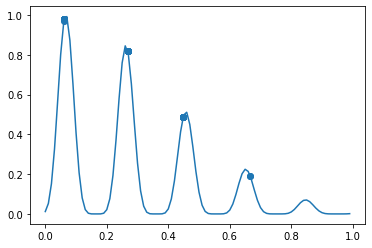
\includegraphics[width=\linewidth]{GA_images/example-transtandal-sin-result.png}
  \captionof{figure}{Result 2}
\end{center}



\captionof{table}{Metric Space}
\begin{tabular}{cccccc}
	\toprule
    $l_{step}$ & $R$ & $C$ & $O_{n}$ & $P_{r}$ & $N_{n}$\\
	\midrule
    1.1 & 0.98 & 2040 & 4.08 & 12.24 & 5.42 \\
    1.6 & 0.98 & 2040 & 5.10 & 13.36 & 5.52 \\
    2.1 & 0.98 & 2040 & 5.18 & 12.06 & 5.12 \\
    2.6 & 1.0  & 2000 & 5.16 & 10.2 & 4.66 \\
    3.1 & 0.98 & 2040 & 4.70 & 9.32 & 4.44 \\
    3.6 & 0.96 & 2083 & 4.5  & 8.22 & 4.12 \\
    4.1 & 0.98 & 2040 & 4.86 & 8.44 & 4.18 \\
	\bottomrule
\end{tabular}

\captionof{table}{$\alpha_{sh}$}
\begin{tabular}{cccccc}
	\toprule
    $\alpha_{sh}$ & $R$ & $C$ & $O_{n}$ & $P_{r}$ & $N_{n}$\\
	\midrule
    1/2 & 0.92 & 2173 & 2.82 & 5.36 & 3.12 \\
    1/3 & 0.92 & 2173 & 4.02 & 6.52 & 3.16 \\
    1.0 & 0.94 & 2127 & 3.66 & 5.32 & 3.14 \\
    2.0 & 0.94 & 2127 & 3.76 & 5.36 & 3.18 \\
    3.0 & 0.98 & 2083 & 3.14 & 5.32 & 3.14 \\
    4.0 & 0.92 & 2173 & 3.48 & 5.28 & 3.12 \\
	\bottomrule
\end{tabular}
\\
\\
Four evaluation criteria are used. 
The first is normalized cost per genetic search, $$C_{n}$$
cost is determinted by the following formula.


\section{Conclusion}
In this paper, three variables of sharing function tensor,$d_{share}$,$\sigma$
was analysed.  The experiment result is measured by five indexes, normalized
search cost, population richness, the number of niche number, the number of
optima. 

\section{Acknowledgements}
This is work was supported by China Schloarship Council(CSC).

%\bibliographystyle{plain}
\bibliography{ga-citation-database}

\end{multicols}
\end{document}
